\documentclass[]{article}

% Imported Packages
%------------------------------------------------------------------------------
\usepackage{amssymb}
\usepackage{amstext}
\usepackage{amsthm}
\usepackage{amsmath}
\usepackage{enumerate}
\usepackage{fancyhdr}
\usepackage[margin=1in]{geometry}
\usepackage{graphicx}
\usepackage{extarrows}
\usepackage{setspace}
\usepackage{float}

%------------------------------------------------------------------------------

% Header and Footer
%------------------------------------------------------------------------------
\pagestyle{plain}  
\renewcommand\headrulewidth{0.4pt}                                      
\renewcommand\footrulewidth{0.4pt}   
\setlength{\parindent}{0em}
\setlength{\parskip}{1em}

%------------------------------------------------------------------------------

% Title Details
%------------------------------------------------------------------------------
\title{Deliverable \#2}
\author{SE 3A04: Software Design II -- Large System Design}
\author{   iSpaceship
        \\ Group 4, T02
        \\
		\\ Pedram Yazdinia, yazdinip
		\\ Will Conry, conrywm
		\\ Torja Istiaque, istiaqum
		\\ Akila Kavisinghe, kavisina
		\\ Xiangxin Kong, kongx9
}

\date{\today}                       
%------------------------------------------------------------------------------

% Document
%------------------------------------------------------------------------------
\begin{document}

\maketitle	

\section{Introduction}
\label{sec:introduction}
% Begin Section

% This section provides a brief overview of the document.

\subsection{Purpose}
\label{sub:purpose}
% Begin SubSection
% \begin{enumerate}[a)]
% 	\item This document will detail some of the design decisions.
% 	%Delineate the purpose of the document
	        
% 	\item Specify the intended audience for the document
% \end{enumerate}

The purpose of this document is to define the software architecture of the computer game iSpaceship from a high-level perspective. The document provides a class analysis, description of the high-level architecture of the system, description of the subsystems, and responsibility cards for each identified class. 

The document is intended for developers as well as business stakeholders, including the Prof, and anyone else interested in a high-level description of the games architecture.

% End SubSectio

\subsection{System Description}
\label{sub:system_description}
% Begin SubSection
 “iSpaceship” is a Rogue-like, turn-based, spaceship battle simulator, video game. The software product will provide the user with an engaging gaming experience where they can build their own spaceship and battle other spaceships. 	The software product will be used for the enjoyment of the user and provide them with a sense of self-accomplishment. The objective is for users to have fun and feel rewarded when they put in the time and dedication to progress in the game. The application should hold interest of users over a long period of time.
% End SubSection

\subsection{Overview}
\label{sub:overview}
% Begin SubSection
This document is divided into five sections, including the above Introduction section.
In section 2, the analysis class diagram is given. This diagram emphasizes the structure of the objects within
the system.
In section 3, the architectural design is described. This section includes descriptions of the overall system
architecture and the divided subsystem architecture.
Finally in section 4, the class responsibility collaboration (CRC) cards are provided. This section outlines
each class required in the system, what it does and its collaborators.
% End SubSection

% End Section

\section{Analysis Class Diagram}
\label{sec:analysis_class_diagram}
% Begin Section
%This section should provide an analysis class diagram for your application.

\begin{figure}[H]
    \centering
    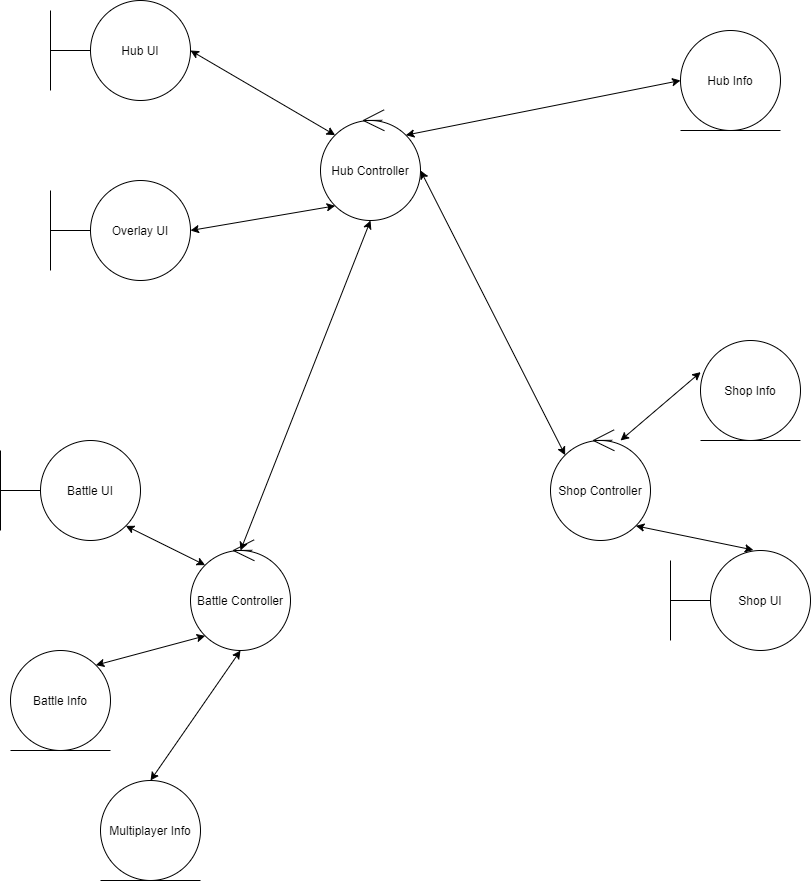
\includegraphics[width=\textwidth]{ClassAnalysis.png}
    \caption{Class analysis diagram for the iSpaceship game.}
    \label{fig:ca}
\end{figure}

% End Section

\section{Architectural Design}
\label{sec:architectural_design}
% Begin Section

%This section should provide an overview of the overall architectural design of your application. You overall architecture should show the division of the system into subsystems with high cohesion and low coupling.
%

\subsection{System Architecture}
\label{sub:system_architecture}
% Begin SubSection

%\begin{enumerate}[a)]
	%\item Identify and explain the overall architecture of your system
	%\item Be sure to clearly state the name of the architecture
	%\item Provide the reasoning and justification of the choice
	%\item Provide a structural architecture diagram showing the relationship %among the subsystems (if appropriate)
%\end{enumerate}
The system will implement the Presentation-Abstraction-Control (PAC) architecture. PAC is an interaction oriented software architecture that breaks a system into a hierarchy of communicating agents. Each agent has three components known as Presentation, Abstraction, and Control. The Presentation component handles interactions with the system interface. The Abstraction component takes care of data manipulation and storage. The Control component is the communication point for the Abstraction and Presentation components. The Control component also communicates between agents. 

PAC architecture was chosen because of the interactive nature of the system being built; iSpacehip requires user input to drive its functionality. PAC allows interactions to be easily designed for due its distribution of system responsibilities. By having a separate presentation, abstraction, and control component user-interactions can be built in a more precise and less-coupled manner. iSpaceship has entity modules that hold information such as players stats and ability information; these can be easily translated to abstraction components. The game also has several boundary classes such as battle and hub which will display screens and received user input; these can be transformed to presentation components. Finally the controller classes such as the Shop or Battle help control and update data from each other; these can be translated to Control components. Finally the hierarchical aspects of PAC can be seen in the system as the top subsystem can be considered to be the Hub. The hierarchical relationship through which the subsystems are connected can be better seen in the package diagram below. 

\begin{figure}[H]
    \centering
    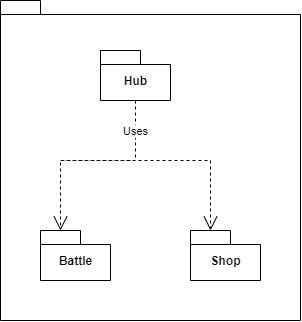
\includegraphics[width=10cm]{StructuralArchitecture.png}
    \caption{Structural architecture diagram for the iSpaceship game.}
    \label{fig:ca}
\end{figure}

% End SubSection

\subsection{Subsystems}
\label{sub:subsystems}
% Begin SubSection



\begin{enumerate}[i]
%	\item Provide a brief description of each subsystem. Be sure to document its purpose and relationship to other subsystems.

    \item \textbf{Hub}: The top level agent of our PAC architecture. It also displays gateways to the main views of the game: the Shop, and the Battle. It also controls the game state and session data and allows the user to save or start a new game.
    
    Also controls the state of the players stats. Including: number of lives, amount of currency, and purchased items. It is stores information for the Shop and Battle subsystems.
    
    \item \textbf{Shop}: Displays the in game item shop where the user can purchase items with in game currency. It controls which items the user can buy and which item the user has by modifying the purchased items in the Hub.
    
    \item \textbf{Battle}: Displays the battle mode of the game where the user battles an opponent. An option is presented for either single player or multiplayer. It records the winners of battles and is responsible for unlocking levels. The player selects abilities to use from another subsystem and they are displayed here. 
    
    Also displays ability options for the user to choose from. It calculates how much damage the player and opponent take each turn using a function of their stats, chosen ability, and a random number. Has a logical component for single and multiplayer.

\end{enumerate}



% End SubSection

% End Section
	
\section{Class Responsibility Collaboration (CRC) Cards}
\label{sec:class_responsibility_collaboration_crc_cards}
% Begin Section


\begin{table}[H]
	\centering
	\begin{tabular}{|p{8cm}|p{5cm}|}
	\hline 
	 \multicolumn{2}{|l|}{\textbf{Class Name:} Hub Controller} \\
	\hline
	\textbf{Responsibility:} & \textbf{Collaborators:} \\
	\hline
	Game Initialization & \\
	\hline
	Main controller of the game & \\
	\hline 
	Accesses game data to transfer to UIs &  Hub UI, Overlay UI\\
	\hline
    Regulates and computes information being relayed by other controllers & Shop Controller, Battle Controller\\
    \hline
    Updates mission results to hub info. & Hub Info, Battle Controller\\
    \hline
    Generates in-game currency & Hub UI, Hub Info\\
    \hline
    Switches game states and gives main control to other controllers & Shop Controller, Battle Controller\\
    \hline
	\end{tabular}
\end{table}


\begin{table}[H]
	\centering
	\begin{tabular}{|p{8cm}|p{5cm}|}
	\hline 
	 \multicolumn{2}{|l|}{\textbf{Class Name:} Battle Controller} \\
	\hline
	\textbf{Responsibility:} & \textbf{Collaborators:} \\
	\hline
    Accesses battle data to transfer to Battle UI. & Battle UI\\
    \hline 
    Computes damage calculations and changes information accordingly. & Battle Info\\
    \hline
    Updates battle results to hub controller. & Hub Controller\\
    \hline
    User is either in multiplayer or in single player story mode. & Multiplayer Info\\
    \hline
	\end{tabular}
\end{table}

\begin{table}[H]
	\centering
	\begin{tabular}{|p{8cm}|p{5cm}|}
	\hline 
	 \multicolumn{2}{|l|}{\textbf{Class Name: }Shop Controller}\\
	\hline
	\textbf{Responsibility:} & \textbf{Collaborators:} \\
	\hline
    Accesses shop data to transfer to shop UI and vice versa. & Shop UI, Shop Info, Hub Controller\\
    \hline
    Updates shop info based on input of shop UI. & Shop UI, Shop Info, Hub Controller\\
    \hline
	\end{tabular}
\end{table}

\begin{table}[H]
	\centering
	\begin{tabular}{|p{8cm}|p{5cm}|}
	\hline 
	 \multicolumn{2}{|l|}{\textbf{Class Name:} Hub UI} \\
	\hline
	\textbf{Responsibility:} & \textbf{Collaborators:} \\
	\hline
    Presents interactive hub interface for user. & Hub controller\\
    \hline 
    Takes input from user to change game states. & Hub controller\\
    \hline 
    Displays spaceship status (level, currency). & \\
    \hline 
    Users can collect generated currencies. &\\
    \hline
	\end{tabular}
\end{table}

\begin{table}[H]
	\centering
	\begin{tabular}{|p{8cm}|p{5cm}|}
	\hline 
	 \multicolumn{2}{|l|}{\textbf{Class Name: } Overlay UI} \\
	\hline
	\textbf{Responsibility:} & \textbf{Collaborators:} \\
	\hline
	General UI to display basic information during all states of the game. & Hub Controller\\
	\hline 
    Acts as a main “desktop” to overlay other UIs. & Hub Controller\\
    \hline
	\end{tabular}
\end{table}

\begin{table}[H]
	\centering
	\begin{tabular}{|p{8cm}|p{5cm}|}
	\hline 
	 \multicolumn{2}{|l|}{\textbf{Class Name:} Battle UI} \\
	\hline
	\textbf{Responsibility:} & \textbf{Collaborators:} \\
	\hline
    Provides interactive battle interface for user. & Battle Controller\\
    \hline 
    Takes in ability input from user. & Battle Controller\\
    \hline
    Displays statistics and battle events. & Battle Controller\\
    \hline
	\end{tabular}
\end{table}

% \begin{table}[H]
% 	\centering
% 	\begin{tabular}{|p{8cm}|p{5cm}|}
% 	\hline 
% 	 \multicolumn{2}{|l|}{\textbf{Class Name:} } \\
% 	\hline
% 	\textbf{Responsibility:} & \textbf{Collaborators:} \\
% 	\hline

% 	\end{tabular}
% \end{table}

\begin{table}[H]
	\centering
	\begin{tabular}{|p{8cm}|p{5cm}|}
	\hline 
	 \multicolumn{2}{|l|}{\textbf{Class Name:} Battle Info} \\
	\hline
	\textbf{Responsibility:} & \textbf{Collaborators:} \\
	\hline
	Contains mission information for all missions. &  Battle Controller\\
	\hline
	Contains damage and other ship stats of current battle. & Battle Controller\\
	\hline
\end{tabular}
	
\end{table}
\begin{table}[H]
	\centering
	\begin{tabular}{|p{8cm}|p{5cm}|}
	\hline 
	 \multicolumn{2}{|l|}{\textbf{Class Name:} Multiplayer Info} \\
	\hline
	\textbf{Responsibility:} & \textbf{Collaborators:} \\
	\hline
	Contains battle information being relayed from multiplayer opponent. & Battle Controller \\
	\hline
	Contains multiplayer stats of the player. & Battle controller\\
	\hline
	\end{tabular}
\end{table}

\begin{table}[H]
	\centering
	\begin{tabular}{|p{8cm}|p{5cm}|}
	\hline 
	 \multicolumn{2}{|l|}{\textbf{Class Name:} Shop Info} \\
	\hline
	\textbf{Responsibility:} & \textbf{Collaborators:} \\
	\hline
	Contains shop entities and respective prices to be displayed in shop. & Shop Controller\\
	\hline
	Keeps tabs on whether item is owned or not. & Shop Controller\\
	\hline
	\end{tabular}
\end{table}

\begin{table}[H]
	\centering
	\begin{tabular}{|p{8cm}|p{5cm}|}
	\hline 
	 \multicolumn{2}{|l|}{\textbf{Class Name:} Hub Info} \\
	\hline
	\textbf{Responsibility:} & \textbf{Collaborators:} \\
	\hline
	Contains all general game information (player name, currency amount, global time, story progression, etc.). &  Hub Controller \\
	\hline
	\end{tabular}
\end{table}

% End Section


\appendix
\section{Division of Labour}
\label{sec:division_of_labour}
% Begin Section
%Include a Division of Labour sheet which indicates the contributions of each team member. This sheet must be signed by all team members.
All members are responsible for 20\% of the work for each milestone.  The work for this document was divided equally amongst all group members.\\
\\\\\\\\\\\\
\begin{tabular}{@{}p{.5in}p{4in}@{}}
Approved: & \hrulefill \\
& Group Member 1 \\\\\\\\\\
Approved: & \hrulefill \\
& Group Member 2 \\\\\\\\\\
Approved: & \hrulefill \\
& Group Member 3 \\\\\\\\\\
Approved: & \hrulefill \\
& Group Member 4 \\\\\\\\\\
Approved: & \hrulefill \\
& Group Member 5 \\\\\\\\\\
\end{tabular}
% End Section

% \newpage
% \section*{IMPORTANT NOTES}
% \begin{itemize}
% %	\item You do \underline{NOT} need to provide a text explanation of each diagram; the diagram should speak for itself
% 	\item Please document any non-standard notations that you may have used
% 	\begin{itemize}
% 		\item \emph{Rule of Thumb}: if you feel there is any doubt surrounding the meaning of your notations, document them
% 	\end{itemize}
% 	\item Some diagrams may be difficult to fit into one page
% 	\begin{itemize}
% 		\item It is OK if the text is small but please ensure that it is readable when printed
% 		\item If you need to break a diagram onto multiple pages, please adopt a system of doing so and thoroughly explain how it can be reconnected from one page to the next; if you are unsure about this, please ask about it
% 	\end{itemize}
% 	\item Please submit the latest version of Deliverable 1 with Deliverable 2
% 	\begin{itemize}
% 		\item It does not have to be a freshly printed version; the latest marked version is OK
% 	\end{itemize}
% 	\item If you do \underline{NOT} have a Division of Labour sheet, your deliverable will \underline{NOT} be marked
% \end{itemize}


\end{document}
%------------------------------------------------------------------------------